\documentclass[twoside,10pt]{article}
\usepackage{shlists}
\usepackage[utf8]{inputenc}
\usepackage[spanish]{babel}
\usepackage[T1]{fontenc}


\usepackage{multicol}
\usepackage{picinpar}

\usepackage{url}
\newcommand{\surl}[1]{{\small\url{#1}}}

\newcounter{vol}
\newcounter{num}
\newcounter{anyo}
\setcounter{vol}{10}
\setcounter{num}{1}
\setcounter{anyo}{2017}
\newcommand{\mes}{Enero}
\usepackage{revisionNLcol}


\title{\ \\ Docencia 2.0\\ \LARGE Lo efímero frente a lo permanente: la tensión en la enseñanza de la informática}
\author{\large Juan Julián Merelo, Fernando Tricas}

\date{}

\AutTit{Docencia 2.0}

\begin{document}
\addtocounter{page}{2}

\maketitle
\vspace*{-5ex}

\begin{multicols}{2}

	Recientemente leíamos que siguen haciendo falta programadores
        (y/o programadoras) de lenguajes obsoletos tales como COBOL,
        Fortran y Clipper \footnote{Major Banks and Parts of Federal
          Gov't Still Rely On COBOL, Now Scrambling To Find IT
          'Cowboys' To Keep Things Afloat,
          \url{https://developers.slashdot.org/story/17/04/10/1441254/major-banks-and-parts-of-federal-govt-still-rely-on-cobol-now-scrambling-to-find-it-cowboys-to-keep-things-afloat}}. Auténticos
        dinosaurios de la informática, o, tratándose de lenguajes,
        latín o cuneiforme, que sobreviven en sistemas que siguen funcionando tal y como fueron diseñados, con algún achaque de vez en cuando. 
Sobreviviendo, por cierto, a otros creados en épocas intermedias que
sí que han sido sustituidos de manera irremediable y, después de haber
sido presentados como la solución de todos nuestros problemas.
Hasta podemos comprender a la dirección estratégica de esas empresas
que no se atreven a emprender un cambio que, seguramente, implicaría
no sólo la actualización de la tecnología sino también cambiar algunas
funcionalidades, añadir otras, y que tiene algunos riesgos evidentes. 

Por otro lado, escuchamos y leemos cómo se acusa a la universidad de no impartir la última tecnología `a la moda' que salvará al mundo de los males que nos atacan.
Por no hablar de cuando afirman que el título universitario es
irrelevante. Que no decimos que no sea posible conseguir un buen
empleo sin título, como prueban los múltiples ejemplos. Pero de ahí a
lanzar a la gente a creer que no tienen que ir a la universidad y que
formarse por su cuenta es una opción para todo el mundo, hay una
cierta distancia. Estudiar una carrera de informática sigue siendo una
de las mejores formas de obtener una experiencia relacionada con y
aprender informática. Evidentemente, el resultado obtenido en la
carrera dependerá de la actitud del estudiante y del lugar donde se
estudie. 

	En medio, toda una panorámica de titulaciones, nuevas y
        antiguas, que cada vez necesitan más de la informática o, como
        mínimo, herramientas informáticas, pero en muchos casos van
        más allá y necesitan la creación o la especificación de
        productos informáticos. Estas titulaciones que tienen
        que confiar en la auto-formación o confiar que el profesorado
        de sus temáticas que sea más competente técnicamente dedique
        algunas sesiones para empezar.

Y en esa tensión estamos.

Creemos que en la universidad se tienen que dar conocimientos básicos,
que permitan tener una carrera posterio larga y fructífera, y
adaptarse a los sucesivos cambios tecnológicos que sin duda vendrán. 
	Pero también pensamos que no sería de recibo hoy en día
        impartir programación utilizando COBOL o Fortran, por llevar
        ese razonamiento hasta sus últimas consecuencias. No parece de
        recibo mantenernos permanentemente en el pasado y no estar
        echando un vistazo a lo que sucede en el mundo para poner
        buenos ejemplos, utilizar tecnologías suficientemente próximas
        a las que parece que se usan en la actualidad, y sobre todo,
        motivar al estudiantado en su trabajo. No se puede dividir a
        las tecnologías, incluyendo sobre todo los nuevos lenguajes de
        programación, en dos categorías: las que damos, que son
        conocimientos básicos y por tanto no importa que no tengan
        ningún uso en el mundo real, y las que no damos, que o bien
        son modas o bien ya las estudiará el alumno cuando termine por
        su cuenta. 

Sobre todo porque en Informática no hay casi nada que permanezca. Una
actualización constante de ejemplos y metodologías transmite la idea
de que (y ya lo decía Heráclito) lo único permanente es el cambio, y
que más valdrá estar en disposición de seguir leyendo, estudiando,
formándose, o rápidamente podemos llegar a ser prescindibles.  Y esto
vale tanto para el estudiante como para el profesor. 

%--------------------------
\noindent\rule{86mm}{1pt}
\vspace{1ex} {\small{\begin{window}[0,r,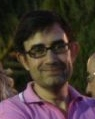
\includegraphics[width = 27mm]{JJM.jpg},] 
\noindent\emph{JJ Merelo} es catedrático de Universidad
en el área de Arquitectura y Tecnología de Computadores, y
actualmente director de la Oficina de Software Libre de la UGR.
Mantiene un blog desde el año 2002, y lo ha utilizado en clase desde
el año 2004; también wikis, agregadores y repositorios de código
como herramientas docente. Últimamente le ha dado por el \textsl{flipped
learning}, de lo que se informará debidamente en esta columna.
\end{window}}}

\medskip

{\small{\begin{window}[0,r,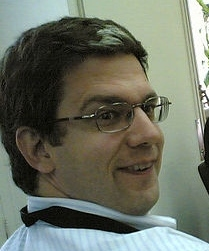
\includegraphics[width = 27 mm]{FTricas1.jpg},]
		\noindent \emph{Fernando Tricas García} es profesor
		titular de Lenguajes y Sistemas Informáticos del Departamento
		de Informática e Ingeniería de Sistemas de la Universidad de
		Zaragoza.  Empezó a estudiar la blogosfera casi cuando aún no
		existía (allá por el año 2002) y a tratar de integrarla en los
		cursos y tareas docentes un poco después.  Ha impartido
		numerosas charlas relacionadas con el tema de la Web 2.0, 
		internet y universidad,\ldots\ 
		Es actualmente Vicerrector de Tecnologías de la Información y
de la Comunicación.   
		\end{window}}}
%-------------------------------------------------




\noindent 
\bigskip

Porque, de esa forma, si han confiado en la universidad para formarse
y adquirir unos conocimientos, a lo mejor más adelante pueden volver a
pensar en nosotros para reciclarse, ponerse al día y, con ese espíritu
de intercambio que venimos defendiendo desde hace tiempo en esta
columna, pedirnos, obligarnos a estar al día y, en definitiva, mejorar
todos. No debemos olvidar que los profesores también tienen una
obligación de transferencia de conocimiento a la sociedad y que si se
usan tecnologías y metodologías actuales en la enseñanza, se dominan y
se ha creado material docente para él, las propias empresas llamarán a
tu puerta para llevar a cabo enseñanza {\em in-house} o
consultoría. La actualización continua de contenidos, en ese sentido,
es una situación donde todo el mundo gana. 


\noindent\emph{Todas las columnas de la serie Docencia 2.0
pueden descargarse en formato LaTeX desde
\surl{https://github.com/ReVision-Docencia-20/Columnas}}

\noindent\rule{90mm}{1pt}

{\small \noindent
\includegraphics[height = 4ex]{../CC.jpg} 2017 JJ. Merelo, F. Tricas. Este artículo es de acceso libre distribuido bajo los términos
de la Licencia Creative Commons de Atribución, que permite copiar,
distribuir y comunicar públicamente la obra en cualquier medio, sólido
o electrónico, siempre que se acrediten a los autores y fuentes
originales}

\end{multicols}
\end{document}
